%%
%% This is file `sample-manuscript.tex',
%% generated with the docstrip utility.
%%
%% The original source files were:
%%
%% samples.dtx  (with options: `all,proceedings,bibtex,manuscript')
%% 
%% IMPORTANT NOTICE:
%% 
%% For the copyright see the source file.
%% 
%% Any modified versions of this file must be renamed
%% with new filenames distinct from sample-manuscript.tex.
%% 
%% For distribution of the original source see the terms
%% for copying and modification in the file samples.dtx.
%% 
%% This generated file may be distributed as long as the
%% original source files, as listed above, are part of the
%% same distribution. (The sources need not necessarily be
%% in the same archive or directory.)
%%
%%
%% Commands for TeXCount
%TC:macro \cite [option:text,text]
%TC:macro \citep [option:text,text]
%TC:macro \citet [option:text,text]
%TC:envir table 0 1
%TC:envir table* 0 1
%TC:envir tabular [ignore] word
%TC:envir displaymath 0 word
%TC:envir math 0 word
%TC:envir comment 0 0
%%
%%
%% The first command in your LaTeX source must be the \documentclass
%% command.
%%
%% For submission and review of your manuscript please change the
%% command to \documentclass[manuscript, screen, review]{acmart}.
%%
%% When submitting camera ready or to TAPS, please change the command
%% to \documentclass[sigconf]{acmart} or whichever template is required
%% for your publication.
%%
%%
\documentclass[manuscript,screen,review,anonymous]{acmart}

%%
%% \BibTeX command to typeset BibTeX logo in the docs
\AtBeginDocument{%
  \providecommand\BibTeX{{%
    Bib\TeX}}}

%% Rights management information.  This information is sent to you
%% when you complete the rights form.  These commands have SAMPLE
%% values in them; it is your responsibility as an author to replace
%% the commands and values with those provided to you when you
%% complete the rights form.
\setcopyright{acmlicensed}
\copyrightyear{2018}
\acmYear{2018}
\acmDOI{XXXXXXX.XXXXXXX}

%% These commands are for a PROCEEDINGS abstract or paper.
\acmConference[Conference acronym 'XX]{Make sure to enter the correct
  conference title from your rights confirmation emai}{June 03--05,
  2018}{Woodstock, NY}
%%
%%  Uncomment \acmBooktitle if the title of the proceedings is different
%%  from ``Proceedings of ...''!
%%
%%\acmBooktitle{Woodstock '18: ACM Symposium on Neural Gaze Detection,
%%  June 03--05, 2018, Woodstock, NY}
\acmISBN{978-1-4503-XXXX-X/18/06}


%%
%% Submission ID.
%% Use this when submitting an article to a sponsored event. You'll
%% receive a unique submission ID from the organizers
%% of the event, and this ID should be used as the parameter to this command.
%%\acmSubmissionID{123-A56-BU3}

%%
%% For managing citations, it is recommended to use bibliography
%% files in BibTeX format.
%%
%% You can then either use BibTeX with the ACM-Reference-Format style,
%% or BibLaTeX with the acmnumeric or acmauthoryear sytles, that include
%% support for advanced citation of software artefact from the
%% biblatex-software package, also separately available on CTAN.
%%
%% Look at the sample-*-biblatex.tex files for templates showcasing
%% the biblatex styles.
%%

%%
%% The majority of ACM publications use numbered citations and
%% references.  The command \citestyle{authoryear} switches to the
%% "author year" style.
%%
%% If you are preparing content for an event
%% sponsored by ACM SIGGRAPH, you must use the "author year" style of
%% citations and references.
%% Uncommenting
%% the next command will enable that style.
%%\citestyle{acmauthoryear}
% Please add the following required packages to your document preamble:
\usepackage{booktabs}

%%
%% end of the preamble, start of the body of the document source.
\begin{document}

%%
%% The "title" command has an optional parameter,
%% allowing the author to define a "short title" to be used in page headers.
\title{Enacting Access: Collaborative Patterns and Dynamic Standard-Making in Ability-Diverse Video Creation Workshops with Blind and Visually Impaired Learners}

%%
%% The "author" command and its associated commands are used to define
%% the authors and their affiliations.
%% Of note is the shared affiliation of the first two authors, and the
%% "authornote" and "authornotemark" commands
%% used to denote shared contribution to the research.
\author{Lan Xiao}

%%
%% By default, the full list of authors will be used in the page
%% headers. Often, this list is too long, and will overlap
%% other information printed in the page headers. This command allows
%% the author to define a more concise list
%% of authors' names for this purpose.
\renewcommand{\shortauthors}{Xiao et al.}

%%
%% The abstract is a short summary of the work to be presented in the
%% article.
\begin{abstract}
Blind and visually impaired (BVI) creators report strong aspirations to make video, yet sustainable training is scarce and mainstream editing applications remain largely incompatible with screen readers. Research prototypes such as script-based accessible editors demonstrate technical feasibility, but they have not translated into deployed training pathways, leaving learners and practitioners reliant on whatever publicly available tools they can adapt. We present an empirical study of how ability-diverse teams learn video creation together, drawing on seven workshops with 10 BVI participants, four tutors, and accompanying support workers across two UK sites between April and July 2025. Combining participant observation, video documentation, post-session reflections, surveys, and post-intervention interviews, we apply multimodal conversation analysis and reflexive thematic analysis to examine how access is enacted moment-to-moment. We identify three interlocking asymmetries that shape collaboration: expertise gaps between video and access pedagogies, fragmentation across tool ecosystems, and incompatibilities between visual-spatial and screen-reader interaction paradigms. Across these asymmetries, four collaborative patterns emerge: haptic mediation, cross-modal translation, task-specific delegation, and peer-to-peer assistance. We propose dynamic standard-making, the situated co-construction of temporary interactional standards between specific collaborators, as a generative reframing of accessibility that complements Universal Design for Learning by accounting for what cannot be designed in advance. We close with implications for inclusive training design, accessible tool development, and pedagogy.
\end{abstract}

\begin{CCSXML}
<ccs2012>
   <concept>
       <concept_id>10003120.10011738.10011773</concept_id>
       <concept_desc>Human-centered computing~Empirical studies in accessibility</concept_desc>
       <concept_significance>500</concept_significance>
       </concept>
 </ccs2012>
\end{CCSXML}

\ccsdesc[500]{Human-centered computing~Empirical studies in accessibility}
%% Keywords. The author(s) should pick words that accurately describe
%% the work being presented. Separate the keywords with commas.
\keywords{Accessible Video Creation, Ability-Diverse Collaboration, Blind and Visually Impaired, Conversation Analysis, Universal Design for Learning, Inclusive Pedagogy}

\received{20 February 2007}
\received[revised]{12 March 2009}
\received[accepted]{5 June 2009}

%%
%% This command processes the author and affiliation and title
%% information and builds the first part of the formatted document.
\maketitle

\section{INTRODUCTION}
Media engagement is more than entertainment for blind and visually impaired (BVI) people, it’s a means of participation, self-representation, and advocacy \cite{emara_its_2025,lyu_because_2024,niu_please_2024}. Research demonstrates that video creation offers BVI individuals significant wellbeing benefits like enhanced social connection, confidence building, and community identity formation, It also enable them to share their stories, educate audiences, and challenge stereotypes despite platform accessibility barriers \cite{seo_understanding_2021,zhang_understanding_2023}.  Yet historically, BVI communities have been underrepresented and sometimes excluded from mainstream media production and cultural venues  due to inaccessible tools, lack of training opportunities, and systemic ableism. \cite{lyu_because_2024,raymond_examination_2024,lyu_i_2024-1}. Unlike text-based blogging or audio-only podcasting, video has emerged as the dominant medium of contemporary digital communication, fundamentally reshaping how we participate in social and cultural life \cite{ha_global_2022}). At the meantime, video creation presents unique challenges and opportunities for BVI creators including inaccessible editing interfaces, inability to verify visual content, and platform-specific barriers.  While the visual-centric nature of video might seem inherently exclusionary, BVI creators have developed innovative approaches to video production that challenge assumptions about who can create visual media and how \cite{seo_understanding_2021,zhang_understanding_2023}. These creators navigate complex workflows involving scripting, audio recording, visual composition, and editing, often developing workarounds for inaccessible tool s while producing content that resonates with both sighted and non-sighted audiences \cite{xiao_understanding_2025}. 

HCI (Human-Computer Interaction) has substantially improved media \textit{consumption} for BVI audiences, including audio description ecosystems, search and viewing support, and design spaces that prioritise non-visual access \cite{aydin_towards_2020, natalie_audio_2024, wang_toward_2021}. In terms of media \textit{creation}, a growing body of work now examines creator practices and proposes tools for accessible production \cite{huh_avscript_2023,lee_altcanvas_2024}. However, practical training programs and capacity-building initiatives for accessible video creation remain largely absent from educational curricula and community-based learning environments.  While self-taught BVI creators have pioneered individual workarounds and shared knowledge through online communities \cite{lyu_i_2024-1,seo_understanding_2021}, the complexity of video production, requiring simultaneous mastery of inaccessible tools, visual verification, and platform-specific requirements, creates barriers that isolated learning struggles to overcome \cite{zhang_understanding_2023}. 

This training gap is particularly significant when considering the collaborative nature of media production. While existing accessibility research often frames BVI creators as individual users navigating inaccessible systems, video creation inherently involves collaboration , from the division of labour required for complex production tasks (scripting, filming, editing, publishing) to the interdependence between visual and non-visual expertise in composing shots, verifying visual content, and ensuring accessibility features \cite{huh_avscript_2023,zhang_understanding_2023,xiao_understanding_2025}. Recent HCI scholarship has begun exploring ability-diverse collaboration, where participants with different abilities work together as interdependent contributors rather than in helper-helped dynamics \cite{bennett_interdependence_2018,xiao_systematic_2024}. Yet we lack empirical understanding of how to structure learning environments that foster genuine ability-diverse collaboration in creative contexts, moving beyond accessibility accommodations toward collaborative interdependence.

To address this gap, we conducted seven workshops designed to teach non-professional video creation skills to participants with visual impairments. Through this case study approach and in line with a participatory action research approach, we investigate two critical research questions: 

\begin{itemize}
    \item \textbf{RQ1:} What barriers/challenges affect video creation education in an ability-diverse team?
    \item \textbf{RQ2:} What collaboration patterns emerge in video creation education within ability-diverse teams and how could them inform the accessible video creation education?
\end{itemize}

\textbf{Contribution Statement: }

This work makes three primary contributions. First, we provide an \textbf{empirical account of the challenges and opportunities} that arise when teaching video creation in ability-diverse settings, offering insights that extend beyond accessibility to fundamental questions about pedagogical design in HCI. Second, we identify specific \textbf{patterns of collaboration that emerge when participants with different visual abilities work together on video projects}, revealing how ability diversity can enhance rather than hinder creative outcomes. Third, we present \textbf{design implications for future tools and curricula settings that support ability-diverse video creation}, grounded in our observations of how participants navigated technological barriers, developed workarounds, and leveraged peer support. These findings contribute to the growing discourse on creative accessibility in HCI while offering practical guidance for researchers and practitioners working to democratize media production.



\section{Related Work}

We organise prior scholarship around three strands that together situate this study: (1) accessible video creation for blind and visually impaired (BVI) creators, where research prototypes have outpaced training infrastructure; (2) ability-diverse collaboration in HCI, where theoretical frames have shifted toward interdependence but empirical attention has centred on workplace settings rather than skill-learning; and (3) Universal Design for Learning and its critiques, which have been read separately from the empirical study of how access is enacted moment-to-moment.

\subsection{Accessible Video Creation: From Prototypes to Practice}

Personal media has become a core route through which BVI creators tell their own stories, build community identity, and challenge stereotypes \cite{emara_its_2025,seo_understanding_2021,brylla_communicative_2024}. Studies of BVI vloggers and bloggers find that creation supports wellbeing, expressive freedom, and visibility in digital spaces, even as platform accessibility remains uneven \cite{seo_understanding_2021,zhang_understanding_2023}. Despite these benefits, structured pathways into video creation are scarce; community surveys and creator studies report video as the most aspired-to and least supported skill area for BVI learners \cite{lyu_i_2024-1,zhang_understanding_2023}.

The barriers to BVI video creation are now well-documented across capture, editing, and publishing. A community study by Zhang et al. \cite{zhang_understanding_2023} found that nearly all BVI participants who had attempted video production encountered breakdowns at editing interfaces, visual feedback, and platform accessibility, with timeline-based interfaces, icon-driven controls, and preview windows particularly poorly supported by screen readers. Huh et al. \cite{huh_avscript_2023} synthesise four recurring challenges: inaccessible visual content, inability to verify visual quality, navigational opacity, and inconsistent screen-reader support. These constraints often push creators toward sighted assistance or restrict editing to the simplest operations \cite{lyu_i_2024-1,xiao_understanding_2025,raymond_examination_2024}.

Recent HCI prototypes propose alternative interaction paradigms that decouple editing from direct visual manipulation. AVscript \cite{huh_avscript_2023} replaces the timeline with a text-based interface that integrates transcripts, scene descriptions, and quality indicators, enabling navigation and selection by content rather than by frame. AltCanvas \cite{lee_altcanvas_2024} offers a tile-based grid for non-visual graphic design, providing accessible feedback for placement and composition. These systems demonstrate technical feasibility, but most remain at the proof-of-concept stage and are not publicly deployed. As a result, learners and practitioners must work with whatever publicly available tools admit partial accessibility, including iMovie, CapCut, and Videoleap, supplemented by AI-assisted aids such as Seeing AI for framing and visual description \cite{xiao_understanding_2025}. Self-taught creators have developed individual workarounds and shared knowledge through online communities \cite{lyu_i_2024-1,seo_understanding_2021}, yet these informal routes assume confidence and digital literacy that many beginners lack.

This split between demonstrated technical feasibility and limited deployment leaves a specific empirical gap. Less is known about how learners and ability-diverse teaching teams negotiate the friction between deployed mainstream tools and research prototypes when those tools sit at the centre of practical training. This study examines that question directly, taking the workshop as its analytical site rather than the individual interface.

\subsection{Ability-Diverse Collaboration in HCI}

A growing body of HCI scholarship reframes disability-related collaboration away from helper--helped dynamics. Wobbrock et al.'s \cite{wobbrock_ability-based_2011} ability-based design argues that systems should adapt to users' specific abilities rather than expecting users to conform to sighted templates, a position later extended to organisational and infrastructural settings \cite{nolte_implementing_2022}. Bennett et al.'s \cite{bennett_interdependence_2018} interdependence framework foregrounds the legitimate labour of coordination, mutual adjustment, and access work in mixed-ability collaboration, recasting access as collectively produced rather than individually granted. Mingus's \cite{mia_mingus_access_2017} concept of collective access offers a parallel formulation grounded in disability justice activism.

Empirical work has begun mapping the patterns through which ability-diverse collaboration operates. Xiao et al.'s \cite{xiao_systematic_2024} systematic review identifies recurrent collaboration patterns (ability sharing, ability combining) and technology roles (ability channel, ability supporter, ability combiner, communication supporter) across the literature. Studies of disabled professionals' collaborative ideation document persistent barriers in shared visual artefacts such as whiteboards and canvases, and argue for practices that externalise structure and surface access needs early \cite{das_that_2024}. Bandukda and Holloway \cite{bandukda_context_2024} examine how mixed-visual-ability dyads share information across context-dependent social interactions, showing that information needs and provision strategies shift moment-to-moment. Due et al.'s \cite{due_distributed_2021} concept of distributed perception describes how perception-related actions are shared across multiple semiotic agents in ability-diverse encounters, with embodied positioning playing a central role in enabling joint achievement.

Despite this progress, much of the empirical evidence draws from established workplace or social settings where roles are relatively stable and participants share prior context. Skill-learning settings present distinct conditions: novices, tutors, support workers, and co-learners occupy partially overlapping roles; the tools themselves are unfamiliar and partially accessible; and pedagogical sequencing constrains when and how access can be negotiated. Earlier studies of inclusive education have noted that group work risks reproducing dependence unless structure redistributes access labour \cite{ahmad_najmee_classroom_2025,barbieri_through_2025}, but few studies attend to the micro-interactional grain at which this redistribution succeeds or fails. This paper extends ability-diverse collaboration scholarship into the skill-learning workshop, asking what collaborative patterns emerge when the tool, the task, and the relationships are all simultaneously under construction.

\subsection{Universal Design for Learning and its Critiques}

Universal Design for Learning (UDL) is the dominant inclusive education paradigm in formal and community settings. Building on the principles of universal design in architecture, UDL specifies that learning environments should provide multiple means of representation, action and expression, and engagement, with the aim of accommodating learner variability without retrofitting \cite{rose_universal_2001,inc_udl_2024}. Empirical evaluations report gains in lesson planning, learner engagement, and instructional flexibility \cite{courey_improved_2013,rao_using_2016}. In BVI media education specifically, the UDL logic underpins arguments for multimodal scaffolds, alternative sensory channels, and accessible artefacts as standard provision rather than individual accommodation \cite{shaheen_exploring_2024,wilkens_using_2025,richard_jackson_audio-supported_2021}.

UDL has nonetheless drawn sustained critique from disability studies scholars who argue that universal design frameworks default to normative assumptions about users and contexts. Dolmage \cite{dolmage_academic_2017} traces how academic UDL reproduces ableist epistemologies even as it claims inclusion, by treating disability as an afterthought to be designed around rather than a generative starting point. Hamraie \cite{hamraie_building_2017} historicises universal design's roots in mid-twentieth-century white, middle-class user models and argues that ``access'' produced under such models embeds the very exclusions it claims to dissolve. These critiques converge on a structural point: UDL operates on a planning logic that presumes modalities can be specified in advance, and that the relevant user variability can be anticipated by designers. What it underspecifies is what happens when, in practice, the available modalities cannot meet a particular learner's needs in a particular moment.

Adjacent to UDL, a body of pedagogical work explores how inclusive maker and media education can be enacted with BVI learners. Hochberg et al.'s \cite{hochberg_supporting_2024} astronomy and computing curricula combine non-visual representations, shared inquiry, and teacher training for mixed-ability classes. Tactile and tangible approaches such as Khalaila and Lazar's \cite{khalaila_streetscape_2025} gamified navigation and Rocha et al.'s \cite{rocha_awareness_2025} tangible programming environments create shared workspaces for mixed-visual-ability collaboration, with explicit turn-taking and aligned metaphors. Sensory-substitution pedagogies extend this further, teaching ``visual'' concepts through structured audio and touch sequences \cite{he_charting_2024}. Across these studies, peer collaboration and co-teaching are repeatedly identified as essential supports for inclusive practice \cite{maesala_overcoming_2024,strogilos_meta-synthesis_2023,travers_collaboration_2024,miyauchi_systematic_2020}, yet the labour through which such supports are sustained, and the conditions under which they fail, remain under-examined.

Across these strands, UDL frames access as something that can be planned ahead of practice, while disability studies frames access as something collectively produced. What is missing is an empirical account of how access is actually enacted in moments where pre-arranged provision fails and learners, tutors, and helpers must construct workable interactional standards together. This paper contributes such an account through what we describe as dynamic standard-making, developed in the discussion in dialogue with the patterns we observe.

\section{BACKGROUND}
\subsection{Project Context}
The [Project Name] project aimed to support BVI participants in developing video creation skills they could continue using in their own creative practice beyond the workshop series. Between April and July 2025 we ran seven structured workshops co-designed and co-delivered with three UK BVI-sector partner organisations (two in [City 1], one in [City 2]), here anonymised as [Partner A], [Partner B], and [Partner C]. The partners supported recruitment, co-facilitation, and integration of the workshops within existing community programmes.

\subsection{Workshop Structure and Curriculum}
Each workshop ran 3--4 hours and followed a consistent session structure. Sessions opened with a brief warm-up that included introductions with visual descriptions, the day's aims, and an outline of activities. Core teaching combined short demonstrations with hands-on practice; in-person sessions had a teaching team of two tutors and one facilitator who circulated to support participants individually, while online sessions were tutor-led with support provided remotely. Sessions closed with a 20--30-minute facilitated reflection focused on challenges, accessibility, and next steps (rationale and procedure in \autoref{sec:design-rationale}). Each workshop was supported by accessible workbooks providing step-by-step VoiceOver-compatible instructions and by teaching slides adapted for screen-reader compatibility.

\begin{figure}
    \centering
    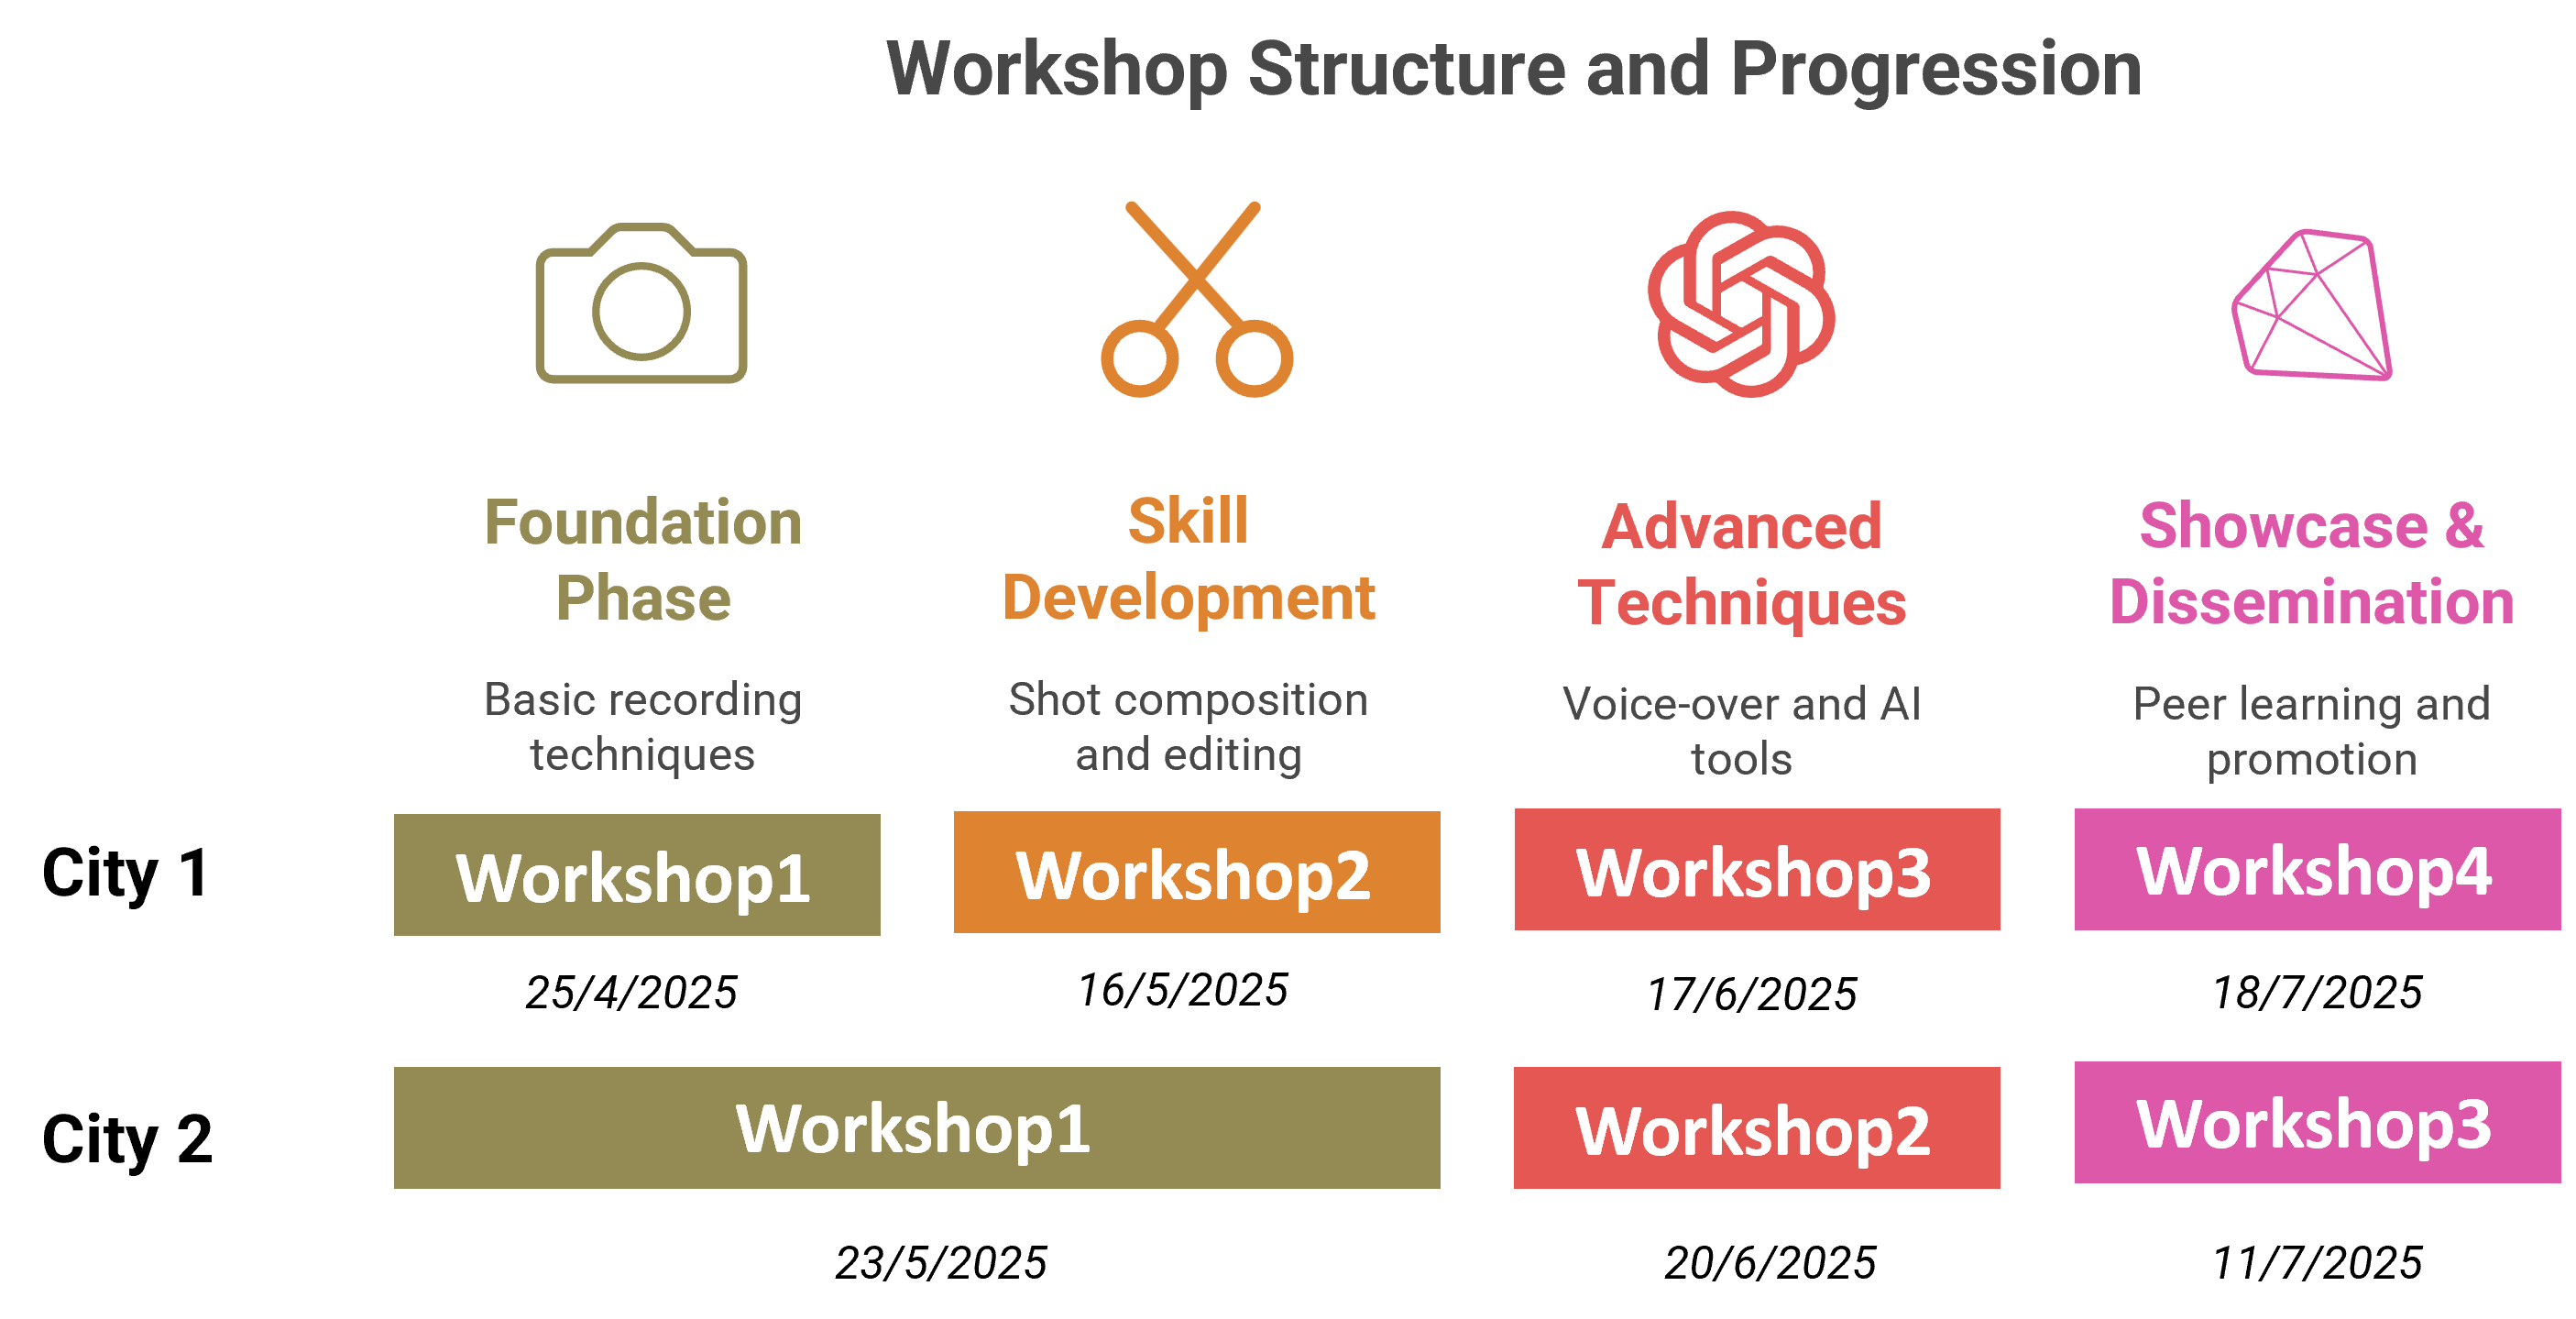
\includegraphics[width=1\linewidth]{Pics/workshop_am.png}
    \caption{Infographic of the four-phase curriculum: Foundation, Skill Development, Advanced Techniques, and Showcase \& Dissemination, with color-coded columns and rows mapping the [City 1] (Workshops 1--4) and [City 2] (Workshops 1--3) sequences.}
    \label{fig:workshop}
    \Description{Infographic with four columns that label the curriculum phases: Foundation Phase (basic recording techniques), Skill Development (shot composition and editing), Advanced Techniques (voice-over and AI tools), and Showcase \& Dissemination (peer learning and promotion). A top row of boxes maps one workshop to each phase for the [City 1] site (Workshops 1-4). A second row shows the [City 2] site configuration where Foundation and Skill Development are combined into Workshop 1, Advanced Techniques is Workshop 2, and Showcase \& Dissemination is Workshop 3.}
\end{figure}

The curriculum followed a scaffolded path (see \autoref{fig:workshop}). The Foundation phase oriented participants to accessible apps and basic equipment (ring lights, tripods, microphones) and covered fundamentals of audio and video capture, with emphasis on confidence in camera pointing, framing through non-visual feedback, and creating simple recordings with music. The Skill-Development phase introduced shot composition (close and wide shots), trimming, basic editing, and music integration, with Seeing AI used as a key tool for framing and recording by providing real-time audio feedback about visual composition. The Advanced Techniques phase covered voice-over narration and AI-assisted graphic generation (stylised selfies, logos, text assets) to extend creative options. The Showcase \& Dissemination phase centred on peer sharing of works-in-progress, advanced prompting strategies, and approaches to online sharing and promotion. Phase-to-workshop mapping differed across the two sites for reasons described in \autoref{sec:design-rationale}.

\subsection{Participants and Teaching Team}

\begin{table}[]
\begin{tabular}{@{}ccccc@{}}
\toprule
\textbf{ID} & \textbf{Age Group} & \textbf{Gender} & \textbf{Vision Profile} & \textbf{Media Creation Experience (0--5)} \\ \midrule
P1          & 40--65              & Female          & Low Vision              & 2                                        \\
P2          & 40--65              & Female          & Low Vision              & 1                                        \\
P3          & 40--65              & Female          & Low Vision              & 2                                        \\
P4          & Over 65            & Male            & Blind                   & 1                                        \\
P5          & 26--39              & Female          & Low Vision              & 3                                        \\
P6          & 40--65              & Female          & Blind                   & 1                                        \\
P7          & 26--39              & Male            & Blind                   & 2                                        \\
P8          & 26--39              & Female          & Blind                   & 1                                        \\
P9          & 26--39              & Female          & Low Vision              & 1                                        \\
P10         & 40--65              & Female          & Blind                   & 1                                        \\
T1          & 26--39              & Male            & Sighted                 & 5                                        \\
T2          & 26--39              & Male            & Sighted                 & 3                                        \\
T3          & 26--39              & Female          & Low Vision              & 4                                        \\
T4          & 26--39              & Female          & Blind                   & 4                                        \\ \bottomrule
\end{tabular}
\caption{Demographics of participants and teaching team. P denotes participant, T denotes teaching team.}
\label{tab:demo}
\end{table}

We engaged 13 BVI participants across two cohorts; three withdrew during the series due to scheduling conflicts or health-related reasons and are not included in the analysis. Recruitment used purposive sampling through partner networks to support diversity in vision conditions, technology experience, and creative backgrounds. Inclusion criteria were self-identification as blind or visually impaired and basic smartphone familiarity; prior video experience was not required. The analytic sample comprises 10 participants (\autoref{tab:demo}; IDs use P for participants and T for teaching team): 8 women and 2 men; ages 26--39 (n=4), 40--65 (n=5), and over 65 (n=1). Vision profiles were evenly split between low vision (n=5) and blind (n=5). Self-rated media-creation experience on a 0--5 scale averaged 1.5 (median 1, range 1--3). Two participants (P3, P4) attended with sighted helpers (\autoref{sec:design-rationale}).

The facilitation team comprised four members in the 26--39 age range with gender balance (two women, two men) and substantial media-creation experience (mean 4.0, range 3--5): a sighted lead tutor (T1), two BVI tutors with video expertise (one low vision (T3), one blind (T4)), and one sighted facilitator providing technical support and visual description (T2). Two team members were drawn from the research team and two were tutor-assistant-trainees nominated by the partner organisations from the [City 1] and [City 2] communities, supporting capacity building within the BVI community.

\paragraph{Sighted helpers.}
Two participants (P3, P4) attended with sighted helpers across the workshops. Helpers were paid support workers or family members. None received role briefing or VoiceOver orientation before the sessions; their digital competence and prior familiarity with the participant varied, and this variation shaped several of the episodes documented in \autoref{sec:results} (see also \autoref{sec:limitations}). Typical helper contributions included device positioning, menu reading, informal coaching, and occasional substitution on visual-verification tasks. We documented helper--participant interactions through field notes and, where helpers consented, through video recording; no formal helper interviews were conducted, for the reasons given in \autoref{sec:design-rationale}. We therefore describe helpers' actions in \autoref{sec:results} as observed rather than as self-reported.

\section{Method}
We used a mixed-methods design that combined participant observation, video-based conversation analysis, and reflexive thematic analysis to examine ability-diverse collaboration in accessible video creation workshops. 

\subsection{Data Collection}

Data collection occurred across seven workshops conducted between April and July 2025, employing multiple methods to capture the complexity of ability-diverse interactions:

\textbf{Participant Observation}: The first author served dual roles as workshop facilitator and participant-observer, documenting interactions through detailed field notes taken during and immediately after each 3–4-hour session. This insider perspective enabled nuanced understanding of both planned activities and emergent collaborative moments. Field notes focused on: (1) instances of cross-ability collaboration, (2) technology-mediated interactions, (3) accessibility barriers and workarounds.

\textbf{Video Documentation}\textbf{:} All workshops were video recorded with participant consent with prior written consent obtained before the first workshop. Recordings captured multiple perspectives including screen recordings of digital activities, wide-angle views of group interactions, and close-ups of specific technical demonstrations. This visual data proved essential for analysing non-verbal communication, spatial arrangements, and the role of sighted guides in facilitating access.

\textbf{Post-Workshop Reflections}\textbf{:} Each workshop concluded with a 20–30-minute guided reflection session where participants discussed their learning experiences, challenges encountered, and collaborative strategies developed. These sessions were audio recorded and transcribed, providing immediate participant perspectives on the workshop activities.

\textbf{Participant Surveys}\textbf{:} Following completion of all workshops, participants completed an online survey (n=10) contains open-ended questions assessing challenges encountered and experiences of collaboration. Survey design followed accessibility guidelines, available in both screen-reader compatible and large-print formats, as well as offered in the form of telephone/Zoom survey.

\textbf{Semi-Structured Interviews}\textbf{:} Two BVI tutors participated in 60–90-minute semi-structured interviews exploring their experiences of the teaching process and cross-ability collaboration. Interview topics included: pedagogical adaptations for mixed-ability groups, observed collaboration patterns, technology's mediating role, and recommendations for future workshops. Interviews were conducted in 1 month after workshop completion, allowing for reflective distance.



\subsection{Data Analysis}

We employed a multi-layered analytical approach suited to our diverse data types:

\textbf{Video-Conversation Analysis} We employed Multimodal Ethnomethodological Conversation Analysis (EMCA) following Due et al. 's work \cite{due_distributed_2021}. The first author manually transcribed selected video clips, then used ATLAS.ti \cite{atlasti_scientific_software_development_gmbh_atlasti_2023} to code multimodal interactions capturing both verbal and embodied elements. This approach helped identify "collaboration episodes" - bounded sequences where participants worked together to achieve specific video creation goals. Each episode was coded for: (1) initiator (BVI participant or sighted instructor), (2) collaboration type, and (3) interaction modality (verbal, visual, tactile).

\textbf{Thematic Analysis} Post-workshop reflections, surveys, and semi-structured interviews were analysed thematically following Braun and Clarke's six-phase approach \cite{braun_reflecting_2019}. Initial codes were generated inductively from participants' descriptions of barriers, facilitators, and collaborative experiences. These codes were then refined through iterative review, resulting in broader themes about accessibility challenges, learning strategies, and support needs.

Following initial separate analyses, we conducted integration sessions where findings from different data sources were synthesized. This process involved mapping collaboration patterns identified through video analysis against themes from interviews and reflections, using interdependence theory as an organizing framework. Contradictions between data sources were explicitly noted and explored as potential insights into the complexity of ability-diverse collaboration.

\textbf{Coding Process}

All initial coding was conducted independently by the first author, then discussed with the research team during regular meeting sessions to review coded excerpts, discuss disagreements, and refine code definitions. Discrepancies were resolved through consensus, ensuring analytical rigor and consistency across the dataset.

\textbf{Integration of Findings}

The video-based EMCA findings and thematic analysis were integrated to produce a comprehensive understanding of BVI video creation education. Collaboration episodes identified through EMCA were contextualized using participants' reflective accounts, while survey responses validated observed interaction patterns. This triangulation revealed how micro-level collaborative practices connected to broader structural barriers in video creation education.

\subsection{Ethical Considerations}
This study received institutional ethics approval [PROTOCOL NUMBER PLACEHOLDER]. Given the visual nature of video workshops and varying vision abilities among participants, we developed a multi-modal consent process including verbal explanation, printed documents, and screen-reader accessible digital forms. Participants could choose their level of data sharing, with options to exclude video footage while maintaining audio participation.
Data management followed institutional guidelines for sensitive data, with video files stored on encrypted servers and access limited to the research team. All identifying information was removed from transcripts, and participants chose pseudonyms for publication.


\section{RESULTS}
\subsection{RQ1. Barriers as Asymmetries in Accessible Video Creation Education}

We synthesize the observed barriers across both in-person ([City 1]) and online ([City 2]) workshops as three interlocking asymmetries: expertise, tools and ecosystems, and interaction paradigms. These asymmetries manifested differently across delivery modes but consistently shaped collaboration across tutor–participant, participant–helper, participant–participant, and tutor–helper relationships. In this section, helpers refer to support workers who accompanied some participants. 

\subsubsection{Expertise asymmetry: video pedagogy vs access pedagogy}

While all tutors possessed strong video production expertise, translating this knowledge into accessible instruction revealed fundamental gaps between visual and non-visual pedagogical approaches. The workshops exposed three critical areas where traditional video pedagogy failed to bridge the accessibility divide.

\textbf{Translation gap between visual and non-visual mental models. }
Tutors who understood timeline editing struggled to convey it non-visually. P3 ([City 2]) remarked, “Some of the words you’re using here, like position the playhead... I’ve got absolutely no idea about the wording.” In [City 1] Workshop 1, a low-vision tutor attempted to guide a blind participant out of the recording feature: “do up swipe like, up and down. And then you can click on the red button, and it will start.” The mixed instruction (gesture plus a colour-based visual referent) illustrates how visual framing persisted even when non-visual navigation was required.

\textbf{Tutor–sighted-guide coordination gap.} Helpers were not part of formal instruction, but they inevitably took on assistance tasks (for example, device positioning, noting steps, reading out menu states). Their effectiveness varied by digital competence and familiarity with the participant. Some pairs coordinated smoothly and provided more support; others contributed little beyond basic prompts. Since helpers received no role briefing or VoiceOver orientation, support quality remained uneven across participants.

\textbf{Documentation and retention gap.} The absence of accessible, stepwise artifacts (e.g., text/audio checklists aligned to VoiceOver and magnifier workflows) shifted learning into short-term memory. As P4 ([City 2]) put it, “I couldn’t find any way for writing them down… it became a memory exercise.” This amplified the pacing asymmetry: without persistent materials, participants could not review or practice between sessions, and tutors had to re-teach procedures in subsequent meetings.
(Following participant feedback from the first workshop, we developed accessible workbooks with step-by-step instructions broken down into granular VoiceOver-compatible steps. This documentation, combined with session slides and audio recordings, significantly improved retention and between-session practice.)

\subsubsection{Tool and Ecosystem Asymmetry: Platform Fragmentation }

\textbf{Application-accessibility incompatibility.} Core editing applications (CapCut, Videoleap) were non-functional with screen readers, blocking blind participants despite their motivation and effort. 

\textbf{Operating system divisions.} The iOS-centric curriculum reduced engagement for Android users. In [City 1], two Android participants could not follow iOS-specific segments. Online, requests for Android coverage (for example, Open Camera) received limited follow-through. Even within iOS, device variations created confusion, for example participants noted iMovie on iPad had more hierarchical menus than on iPhone.

\textbf{Workflow-level friction rather than app-level absolutes.} Rather than a single app being strictly unusable, participants encountered practical breakdowns when screen reader navigation and editor workflows did not align in-session, which led to abandoned steps and detours. During [City 1] Workshop 2, P6 attempted to trim a video clip in iMovie. The participant could navigate to the timeline using VoiceOver, which announced "timeline, adjustable" when reached. However, determining the playhead's exact position required visual feedback that VoiceOver couldn't provide.
(80\% of our participants, sustainability, limitation, )

\subsubsection{Interaction paradigm asymmetry: Competing Navigation Models}
Fundamental differences between visual touch and screen reader gesture models created persistent collaboration barriers.

\textbf{Dual instruction burden. }Each technique required parallel explanation across paradigms. Low-vision participants could follow “press the red button,” while blind participants needed instructions grounded in element order and audio labels. Attempting both tracks simultaneously slowed progress and introduced confusion. Online, this surfaced as focus-control difficulties, for example P4 ([City 2]) noted, “with my four-minute video, it’s just whizzing through it a bit.”

\textbf{Cognitive load from paradigm switching.} Translating each step across visual–spatial references (“press the red button”) and non-visual traversal (element order + labels via VoiceOver) demanded continuous remapping by blind participants,and by tutors narrating both tracks. In noisy rooms, earphone use to hear VoiceOver improved access but further limited overheard feedback and ad-hoc assistance, compounding cognitive effort.

\textbf{Helper–participant navigation disconnect. }With screen curtain enabled, displays were not visible by design, eliminating visual guidance routes for helpers. Even with screen curtain off, helpers’ mental models did not match VoiceOver’s gesture grammar, limiting them to minimal prompts such as “next one,” “confirm,” and “go back.” In louder in-person rooms, several screen reader users used earphones to hear VoiceOver. This improved their own access but further limited the possibility of ad hoc support from tutors or nearby peers who could not hear the screen reader feedback.

\textbf{Group-level access conflicts. }Mixed-ability groups faced competing needs that could not be simultaneously met. Magnifier-optimized instructions confused screen reader users, while detailed verbal descriptions for blind participants slowed those with residual vision. Participants recognized this tension: "It's always difficult when you've got a mixture of totally blind and partials... trying to adjust to the different needs." The feedback to create "two different groups... one only screen readers, one uses magnifiers" acknowledged these fundamental incompatibilities.

\subsubsection{Delivery Mode Trade-offs: Co-located vs Remote }
\textbf{Co-located affordances and constraints.} In-person sessions enabled tactile and embodied learning with cameras, rigs, and phones. Participants could “touch it and use it,” and tutors could adjust posture, framing, or grip. These benefits required intensive individualized facilitation that was difficult to scale in moments of divergence across access modalities.

 \textbf{Remote affordances and constraints.} Online sessions supported replay and self-pacing but limited physical device demonstration. Certain concepts, for example stabilization or tripod setup, were hard to convey without hands-on interaction. File transfer remained a recurring barrier, with cloud storage failing unpredictably for some participants and preventing cross-device sharing at critical moments.

\subsection{RQ2. Collaborative patterns emerge in ability-diverse video creation education }

Our analysis reveals that different combinations of vision abilities produce distinct collaborative strategies and interaction patterns. Rather than viewing visual impairment as an individual attribute, we found that collaborative dynamics emerged from the specific configurations of abilities within dyads and triads. Following our analytical approach, we identified four primary patterns, each with characteristic interactions, temporal organizations, and collaborative strategies that fundamentally shaped learning experiences in ability-diverse workshops.

 \begin{figure}
     \centering
     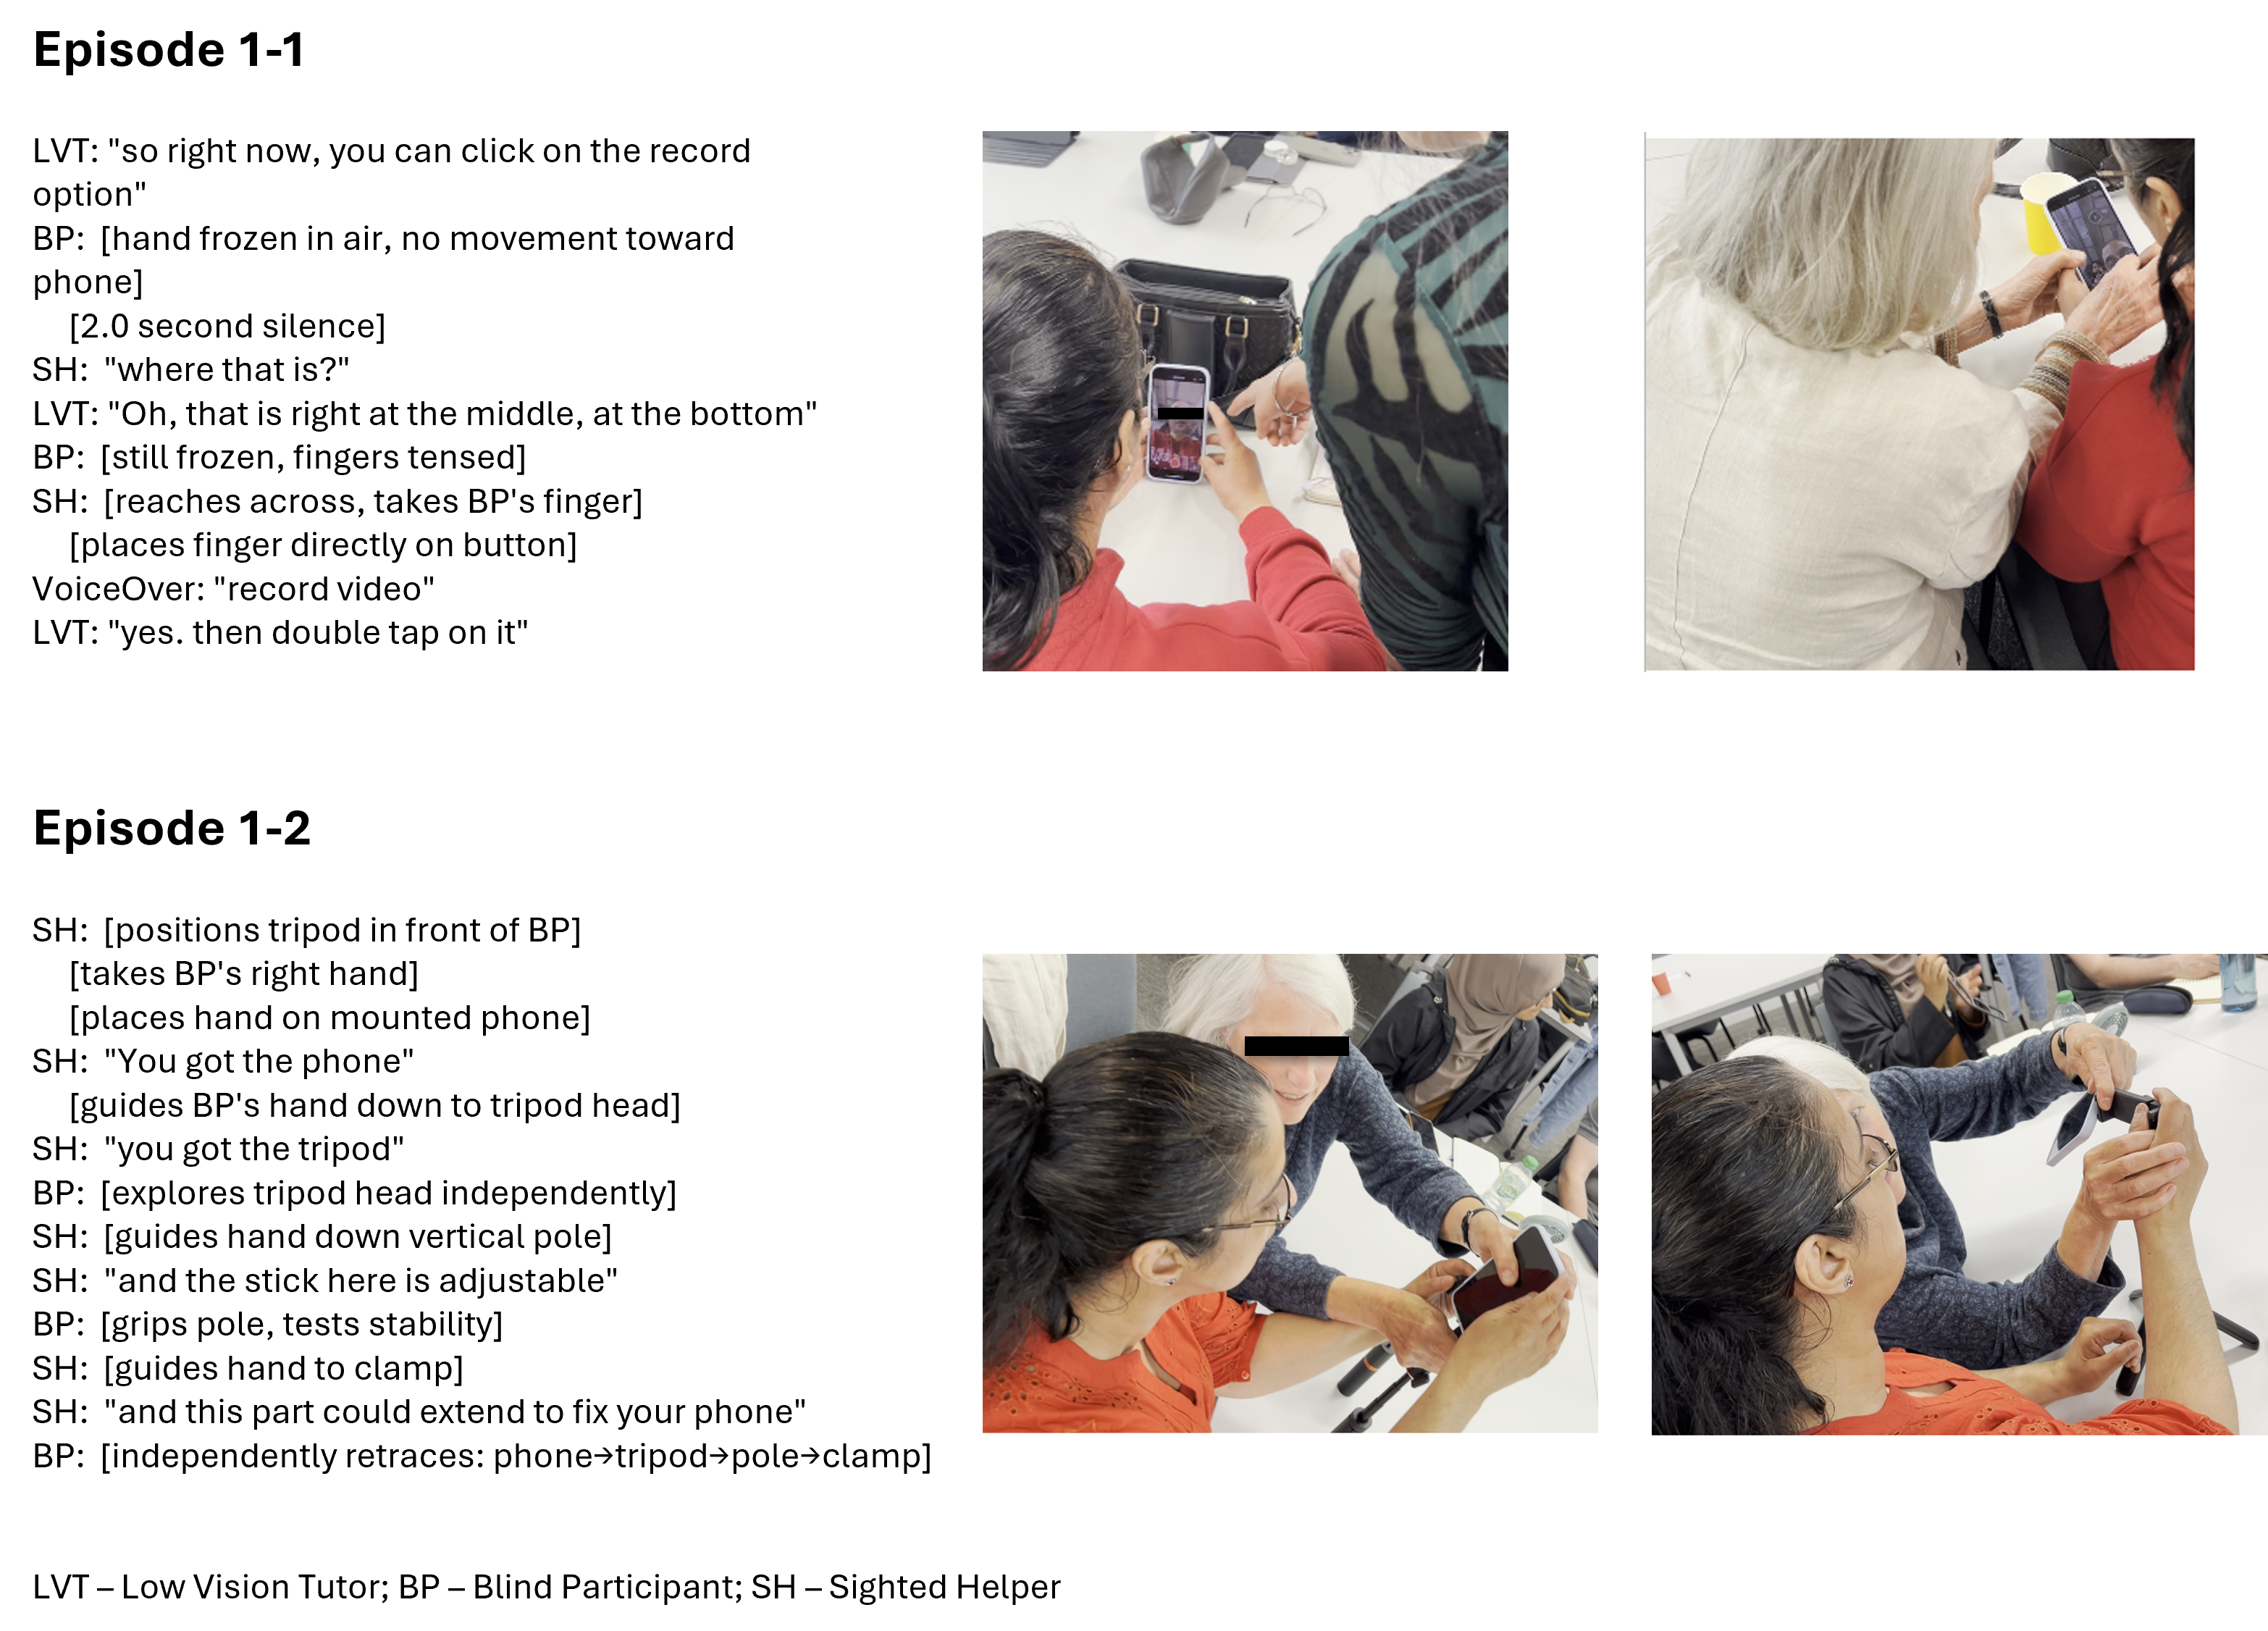
\includegraphics[width=1\linewidth]{Pics/Pattern_1.png}
     \caption{Collaborative patterns: : Direct haptic mediation (Episode 1 \& Episode 1-2)}
     \label{fig:paatern1}

\Description{Four-photo collage from a hands-on mobile-video workshop. Top left: a participant records a short clip of an older woman using a smartphone while others observe. Top right: an older woman guides two participants as they look at a phone together. Bottom left: two participants position a phone in a small clamp and discuss settings. Bottom right: participants fasten a phone onto a wrist-mount for wearable recording. The scenes emphasise peer instruction and shared manipulation of devices. }
 \end{figure}

\subsubsection{Pattern 1: Direct Haptic Mediation }
When blind and sighted (or partially sighted) participants collaborated, interactions consistently followed a pattern of direct haptic mediation, systematically bypassing verbal description in favour of physical guidance.

\textbf{Episode 1-1: Physical Placement Over Verbal Direction. }In the recording button episode from the [City 1] workshop ( \autoref{fig:paatern1}), we observe how verbal spatial descriptions fail to provide actionable information for blind participants, leading to immediate haptic intervention. The interaction begins with what appears to be a straightforward instruction from a low vision tutor: "so right now, you can click on the record option." However, this instruction lacks any spatial reference that would enable the blind participant to locate the button. The participant's response,hand frozen in air with no movement toward the phone,materially demonstrates complete spatial disorientation. The 2.0-second silence that follows is not merely a pause but what conversation analysts term a "dispreferred response" marker, indicating trouble in the interaction.

A sighted helper sitting beside the participant recognizes this trouble and intervenes with the critical question: "where that is?" This question does more than request information; it explicitly identifies the missing element in the tutor's instruction. The tutor's response:” Oh, that is right at the middle, at the bottom" provides visual-spatial coordinates that would be immediately actionable for a sighted person. 

However, the blind participant's continued frozen posture and tensed fingers reveal that these visual coordinates remain non-actionable. The visual-spatial framework of "middle" and "bottom" requires a mental model of the screen as a two-dimensional plane with established directional orientational, model that depends on visual access for its construction and maintenance. As Figure 1 shows, the sighted helper's immediate response represents a complete bypass of verbal-spatial description through direct finger placement on the button, followed by successful VoiceOver confirmation and the participant's independent double-tap execution. 

\textbf{Episode 1-2: Systematic Tactile Mapping. }For physical equipment introduction, blind-sighted dyads developed highly structured exploration patterns that revealed sophisticated understanding of non-visual spatial learning. In the tripod familiarization sequence (\autoref{fig:paatern1}), the sighted helper employed a methodical approach that systematically constructed a mental map through guided touch. The helper began by positioning the tripod directly in front of the blind participant, then took their right hand and placed it on the phone already mounted, providing the verbal anchor "You got the phone."

The exploration continued systematically downward,from phone to tripod head to vertical pole,with each component verbally labelled as the participant's hand made contact. Notably, between each guided segment, the blind participant engaged in independent exploration: fingers examining the tripod head's texture and joints, hands gripping the pole to test stability, and rotating the adjustment ring experimentally. These moments of autonomous investigation, interspersed between guided movements, demonstrate active learning rather than passive reception. The sequence concluded with the participant independently retracing the entire path from phone to clamp, confirming successful spatial map construction through haptic channels.
 \begin{figure}
     \centering
     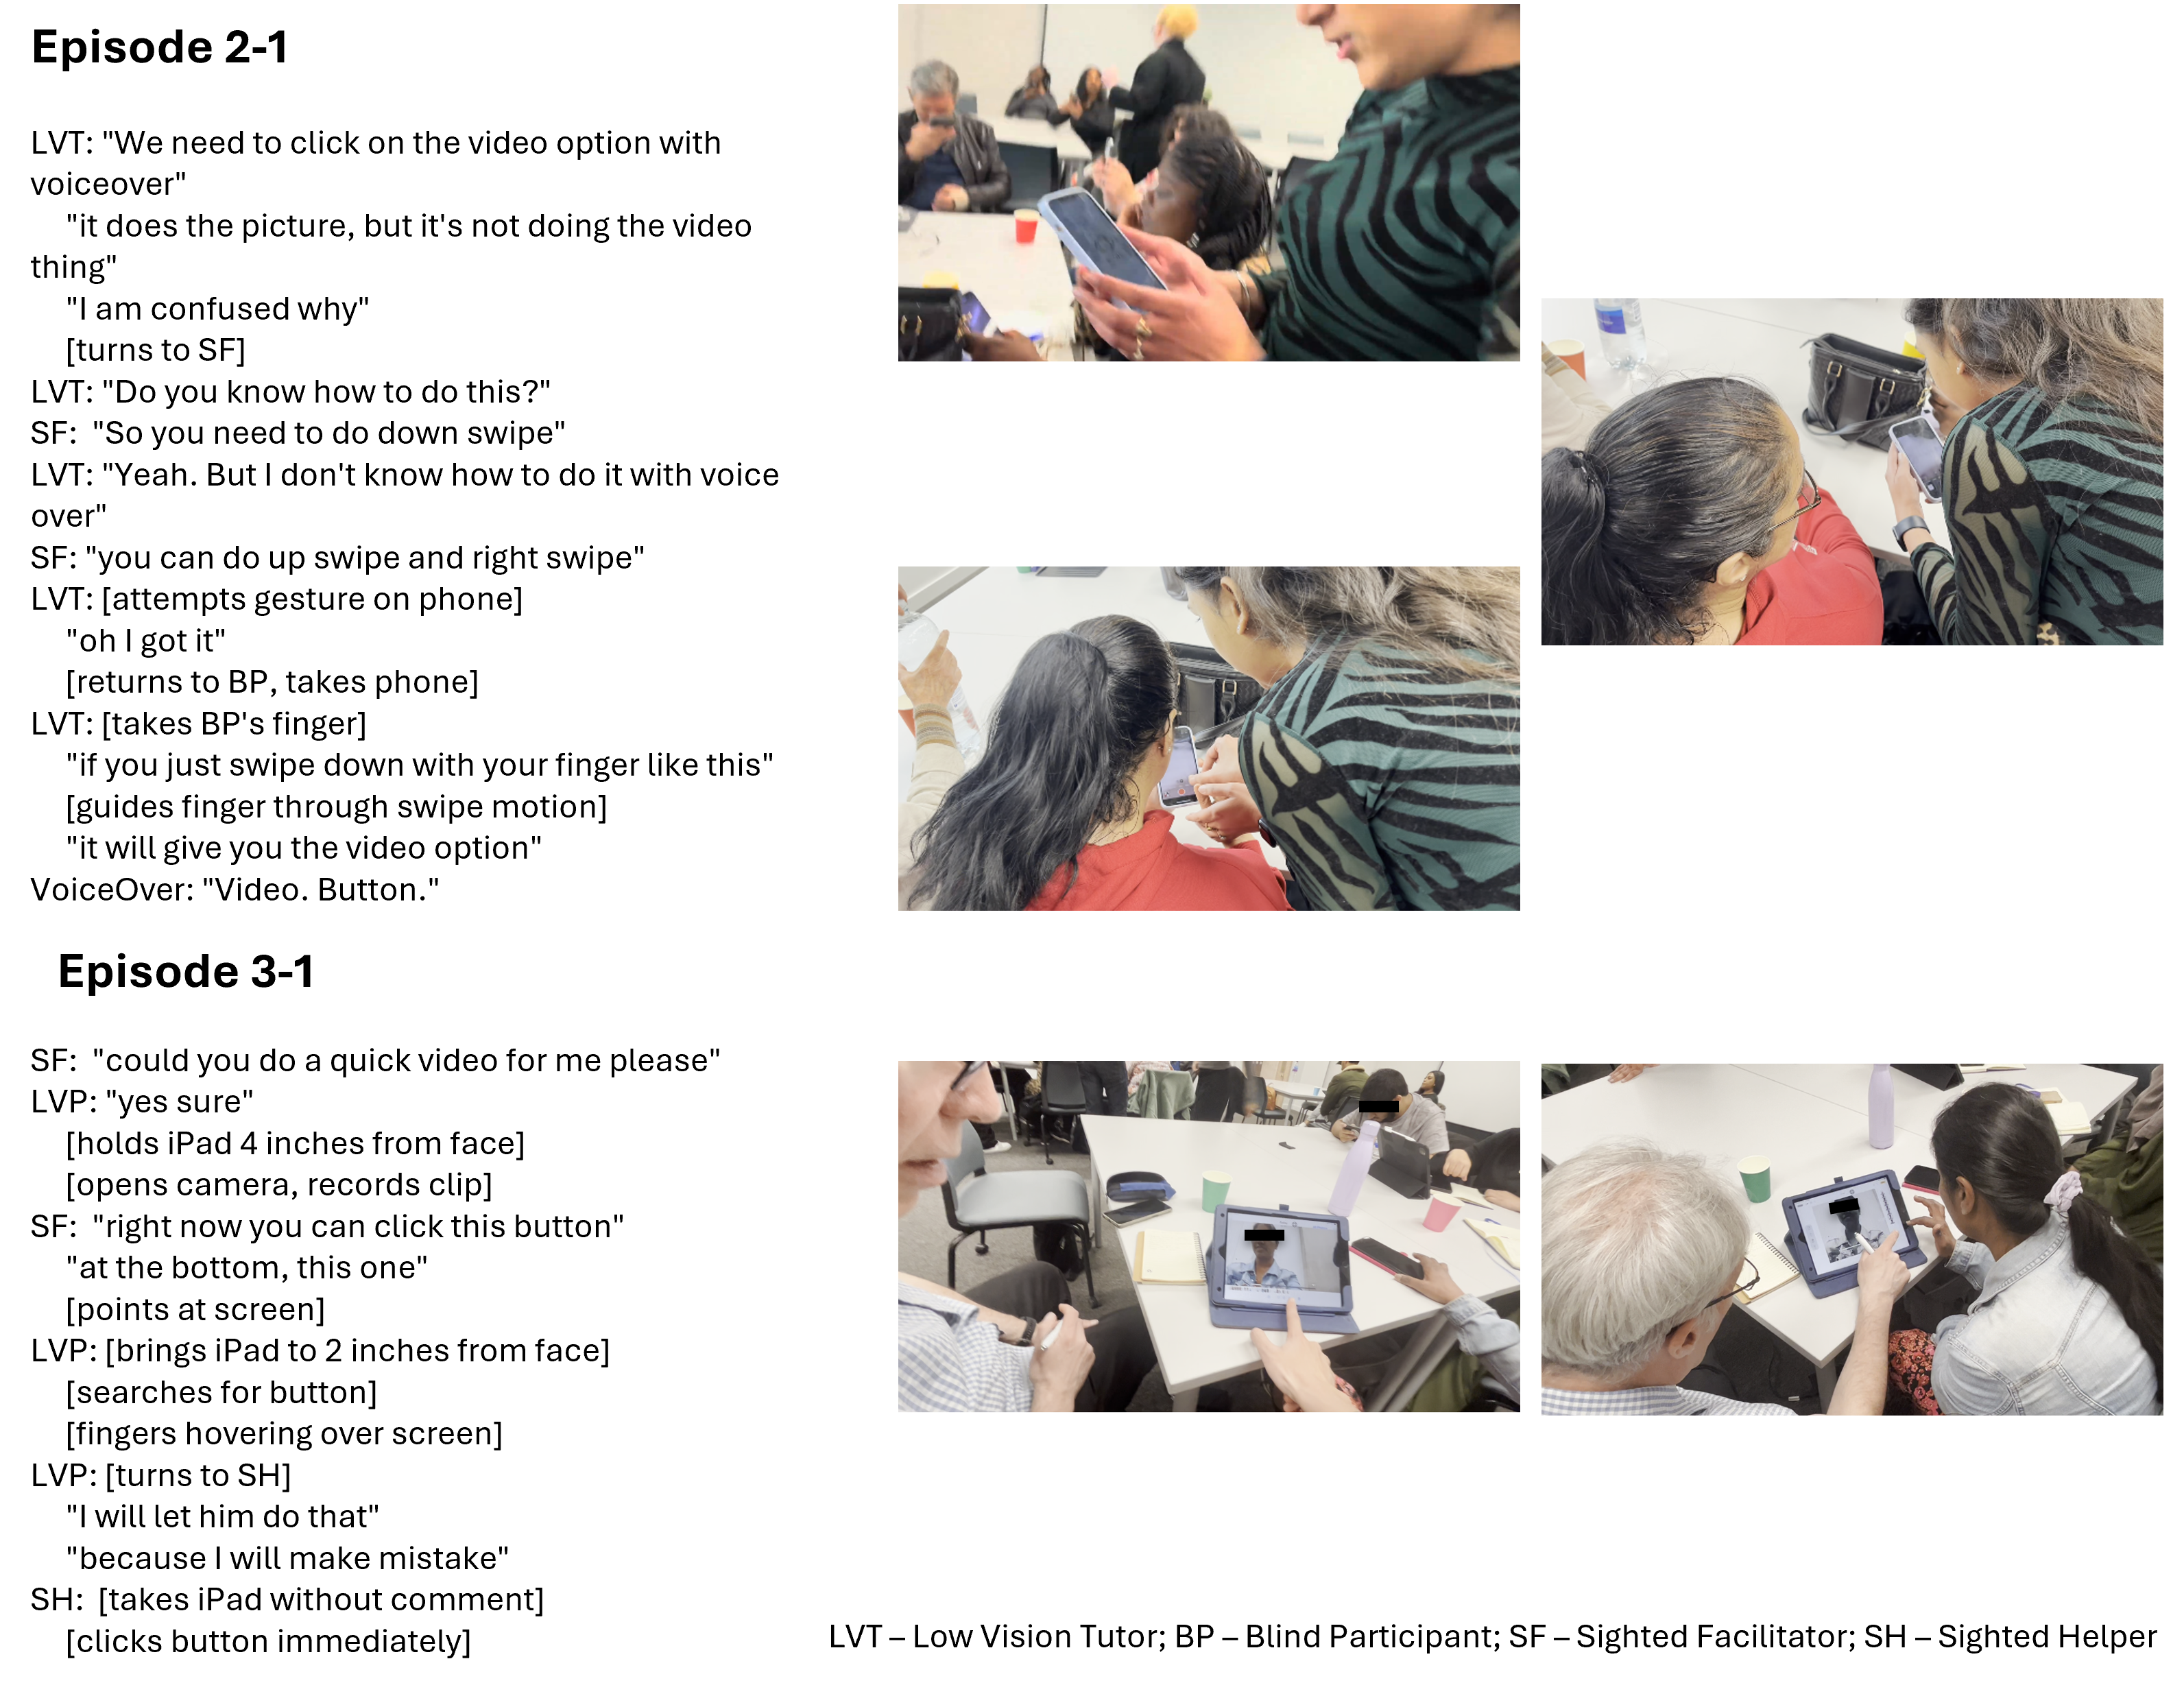
\includegraphics[width=1\linewidth]{Pics/Pattern_2.png}
     \caption{Collaborative patterns: Cross-modal translation (Episode 2-1) and task-specific delegation(Episode 3-1) }
     \label{fig:paatern2}

\Description{Five-photo collage showing collaborative exploration of mobile filming and editing. Top left: wide view of a classroom with people at tables; a facilitator checks a participant’s phone. Top right: two women review footage on a phone. Centre: a close view of a participant pointing to options on another person’s phone. Bottom left and bottom right: pairs review clips on a tablet, with one person pointing to the on-screen timeline. Images highlight peer learning, reviewing recordings, and simple edits on phones and tablets.}
 \end{figure}
\subsubsection{Pattern 2: Cross-Modal Translation}
When dyads reach their limit, they often recruit a third party. This strategy appears when helpers mark the boundary of their current knowledge and invite joint problem solving without abandoning their role. The newly added collaborator typically contributes a missing rule or gesture, which then must be translated into VoiceOver-compatible action for the blind participant.

\textbf{Episode 2-1: }In the VoiceOver mode-switch scene (\autoref{fig:paatern2}), the low-vision tutor identifies the current state (“picture” rather than “video”), then states the procedural gap: “it is not doing the video thing. I am confused why.” She then went for the sighted facilitator for help. a sighted facilitator provides the procedural key as gesture talk (“you need to do down swipe”). The low-vision tutor differentiates concept and implementation (“I do not know how to do it with VoiceOver”). After a brief, mid-air demonstration with verbal accompaniment (“you can do up swipe and right swipe”), the tutor practices and signals uptake (“oh I got it”). Only then can they relay the instruction haptically, taking the participant’s finger and guiding the on-screen motion while narrating the VoiceOver outcome (“if you swipe down, it will give you the video option”). The low-vision collaborator operates as a modality relay: sighted gestural instruction becomes embodied skill, then becomes tactile coaching aligned with the screen reader.

\subsubsection{Pattern 3: Task-Specific Delegation Protocols}
Low-vision participants actively manage independence and accuracy, switching between solo action and targeted hand-off.

\textbf{Episode 3-1: }In the iPad editing episode (\autoref{fig:paatern2}), a low-vision participant confidently records a short clip with the device 4 inches from their face. When asked to “click this button, at the bottom, this one,” the device shifts closer, to roughly 2 inches, indicating increasing visual strain for smaller, less familiar controls. Fingers hover near the region, suggesting approximate knowledge but risk of error. The participant then states, “I will let him do that because I will make mistake,” and hands the device to a sighted helper, who selects the control without negotiation. Delegation is framed as error prevention rather than inability, preserving agency while meeting the task requirement.

\subsubsection{Pattern 4: Peer-to-Peer Assistance  }
During remote workshops, participants with advanced technical skills emerge as peer coaches, providing targeted procedural guidance that bridges knowledge gaps. These peer experts demonstrate deep understanding of both the technology and the accessibility features, offering precise instructions that preserve learner agency while ensuring task completion.

\textbf{Episode 4-1: Spatial Navigation Expertise}
When participants struggle with camera mode switching, a blind participant with extensive iPhone experience, provides precise spatial guidance: "You go to the bottom right hand corner. And that is where... if you wish to change the video, you go slightly further up than the shutter. And that's where you will find the mode button" He then details the gesture mechanics: "It's a flick. You do a vertical flick, so you put your finger on it and then you do a vertical flick either up or down." This demonstrates how blind experts develop and share detailed mental maps of interface layouts, translating spatial relationships into actionable instructions. He also corrects misconceptions about navigation methods, demonstrating his deep VoiceOver expertise: "May I just say when it comes to the iPhone, there's no swiping. You go to the bottom right hand corner, you'll see, back camera or front. All you do is just double tap on it and it will change" His correction shows how peer experts understand the distinction between different navigation modes and can guide others to the most efficient interaction patterns.

\section{DISCUSSION}
Our investigation into how BVI individuals learn video creation through structured workshops reveals fundamental challenges in translating visual media production into accessible pedagogy.  By examining barriers and collaborative patterns, we identify how access is achieved not by universal solutions, but through dynamic, localized negotiations among individuals with different sensory abilities . We organize our conversation around three main themes: (1) what inclusive video creation education requires in terms of materials, pacing, and instructional approaches, (2) how collaboration emerges through dynamic negotiations between participants with different sensory abilities, and (3) how distributed expertise across peer networks can compensate for individual knowledge gaps.

\subsection{Implications for Inclusive Video Creation Education}

\subsubsection{Reframing Access Through Interaction Design }
Our findings demonstrate that the fundamental challenge in ability-diverse video creation education lies not in the epistemic differences between visual and non-visual ways of knowing, but in the interaction asymmetries these differences create. While participants with different vision profiles inevitably construct distinct mental models of video creation, for example, visual-spatial for sighted and low-vision users, sequential-temporal for screen reader users, these epistemic frameworks need not be barriers to learning. As our collaborative patterns reveal, participants successfully navigated these differences when interaction barriers were addressed through haptic mediation (Pattern 1) and cross-modal translation (Pattern 2).

This distinction between epistemic and interaction asymmetry extends Wobbrock et al.'s ability-based design framework \cite{wobbrock_ability-based_2011} by suggesting that educational technologies should not attempt to normalize different ways of knowing but rather create interaction bridges between them. For instance, when the low-vision tutor in Episode 2-1 served as a "modality relay," translating gestural instructions into VoiceOver-compatible actions, they preserved the integrity of both epistemic frameworks while enabling successful task completion. This suggests that future video creation tools designed for education should prioritize interaction flexibility over content uniformity, allowing multiple valid pathways to achieve creative goals.

\subsubsection{From Individual to Dyadic Pedagogies }
Perhaps our most significant finding concerns the reconceptualization of the learner unit in accessible media education. Rather than treating BVI participants as individual learners requiring accommodation, our data reveals the collaborative dyad as a more effective pedagogical unit. Episodes 1-1 and 1-2 demonstrate how helper-participant pairs developed sophisticated collaborative protocols that went beyond simple assistance to create what Bennett et al. term "interdependence \cite{bennett_interdependence_2018}."  However, our findings extend this framework by showing that interdependence can be explicitly taught and scaffolded rather than emerging spontaneously.

Educating collaborative dyads would involve several strategic shifts. First, orientation sessions should address both participants and their support workers together, establishing shared vocabulary and interaction protocols. Second, curricula should include explicit instruction in cross-modal communication strategies, teaching helpers how to provide spatial information through haptic guidance and verbal description that aligns with screen reader navigation. Third, assessment criteria should evaluate collaborative achievement rather than individual mastery, recognizing that distributed expertise represents a valid and valuable form of media literacy. This approach transforms support workers from peripheral accommodations into integral pedagogical partners, a shift that acknowledges the reality of collaborative creative practice in professional media production.

\subsubsection{Infrastructural Requirements for Ability-Diverse Learning }
The tool and ecosystem asymmetries we identified point toward specific infrastructural requirements for sustainable video creation education. Our participants encountered not app-level barriers but workflow-level friction when screen reader navigation and editing paradigms misaligned. This suggests that accessible video education requires standardized, cross-platform tools that maintain consistency across devices and operating systems. Web-based applications present a promising approach for addressing platform fragmentation, as they could provide uniform interfaces across iOS and Android while leveraging established web accessibility standards.

However, given the current absence of fully accessible video editing platforms, education programs must develop systematic workarounds. Our findings suggest these workarounds should be formally documented in multiple accessible formats—text descriptions for screen reader users, visual guides for magnifier users, and audio walkthroughs for review between sessions. The documentation gap P4 identified ("it became a memory exercise") could be addressed through persistent, multi-modal learning artifacts that participants can reference during independent practice.

\subsubsection{Cultivating Peer Expertise Networks }
The emergence of sophisticated peer teaching in our remote sessions (Pattern 4) reveals an underutilized resource in accessible media education. The "flatter" structure of online workshops, where participants occupied equal visual space in gallery view without the hierarchical arrangement of traditional classrooms, facilitated peer-to-peer knowledge exchange. Episodes 4-1 demonstrate how BVI participants with advanced technical skills provided precise spatial guidance and cross-version label mapping that preserved learner agency while ensuring task completion.

This peer expertise should be intentionally cultivated through structured opportunities for knowledge sharing. Mixed-experience cohorts, where novice and advanced BVI creators learn together, can create natural mentorship relationships. Formal peer teaching roles, where experienced participants demonstrate specific techniques or troubleshoot common problems, validate BVI expertise while providing relatable instruction. Remote learning environments particularly support this approach, as they eliminate physical barriers to peer assistance while maintaining equal participant presence. Additionally, implementing screen sharing and remote control capabilities in online sessions could address the limitation we observed where helpers could only provide verbal guidance, extending the haptic mediation strategies successful in face-to-face contexts to digital environments.

\subsection{From Universal Design to Dynamic Standard-Making}
Our results challenge the assumption that universal design can sufficiently accommodate ability-diverse learning environments. The three asymmetries we identified: expertise, tools, and interaction paradigms, demonstrate that participants function within fundamentally divergent epistemic frameworks based on their sensory modalities. This corresponds with theories of embodied cognition \cite{varela_embodied_1991,wilson_six_2002} illustrate that various sensory modalities engender unique cognitive frameworks.

The visual-touch, visual-assisted, and voice-tactile modes we observed represent not simply different ways of accessing the same information, but different ways of knowing and interacting with the world. This aligns with Thieme et al.'s research \cite{thieme_enabling_2017} on how individuals with visual impairments navigate their capabilities in social settings, and it expands upon Moser's assertion that disability is manifested differently across socio-material situations \cite{moser_disability_2006}.

This epistemic variety poses a challenge to the concepts of Universal Design for Learning (UDL) \cite{inc_udl_2024,rose_universal_2001}, which assume that various modes of representation, interaction, and expression may accommodate all learners. Although UDL has advanced inclusive education significantly \cite{courey_improved_2013,rao_using_2016}, our research indicates that its framework may unintentionally enforce a unique epistemic standard. Similar critiques have emerged from disability studies scholars who argue that universal design often defaults to normative assumptions \cite{dolmage_academic_2017,hamraie_building_2017}. 

Instead, our collaboration patterns illustrate what we refer to as "dynamic standard-making": the creation of temporary, localized standards between specific individuals that enable particular learning moments. This idea is based on Suchman's situated action theory \cite{suchman_human-machine_2006}, It says that standards come from practice, not the other way around, also Wobbrock et al.'s ability-based design framework \cite{wobbrock_ability-based_2011}, which argues that systems should adapt to users' abilities rather than requiring users to adapt to systems. Our findings extend this by showing that in collaborative contexts, the "system" itself is co-constructed through practice. When participants engaged in haptic mediation or cross-modal translation, they were not just adapting to each other's abilities but actively constructing what Lave and Wenger call "communities of practice" \cite{lave_situated_1991} with their own internal logics. These temporary standards represent ability-based design enacted socially, where the collaborative dyad or triad creates custom interaction protocols that leverage each person's specific abilities in that moment.

\subsection{The Distribution of Access}
Building on Goodwin's concept of "co-operative transformation zones," \cite{goodwin_co-operative_2013} we see how participants progressively transform the substrate of prior interactions to create new forms of collaboration. Each workshop session builds upon resources and techniques developed in previous sessions, creating what Goodwin calls an "accumulative" process central to human culture and knowledge.

The progression from direct haptic mediation to sophisticated peer teaching exemplifies what Due terms "distributed perception" \cite{due_distributed_2021}: where perception-related actions are shared among agents who co-operate to accomplish activities that could not be achieved individually. In our workshops, BLV participants relied on sighted participants' visual perception, but crucially, this was not passive dependency. Instead, as Due demonstrates, distributed perception requires active "positioning for perception" \cite{goodwin_participation_2007}, where participants must bodily and technologically position themselves to enable perception-related actions.

This distributed model challenges traditional special education approaches where expertise flows unidirectionally from teacher to student \cite{giangreco_students_2002}. Instead, we observed what Bennett et al. term "interdependence," \cite{bennett_interdependence_2018} where all parties contribute essential knowledge. The evolution of collaborative patterns we documented suggests that groups develop what Akkerman and Bakker call "boundary crossing competence," \cite{akkerman_boundary_2011} becoming increasingly skilled at navigating between different epistemic frameworks. 

This distributed model contrasts with research on paraprofessional support showing that traditional helpers often create dependency rather than independence \cite{causton-theoharis_increasing_2005}. Our observations align better with Bennett et al.'s interdependence framework \cite{bennett_interdependence_2018} and recent work on collective access \cite{mia_mingus_access_2017}, where access is understood as a collective responsibility rather than individual accommodation.

\section{CONCLUSION}
This paper examined ability-diverse collaboration in video creation workshops for blind and visually impaired communities, revealing fundamental challenges to prevailing models of inclusive education and accessible technology design. Through detailed analysis of seven workshops combining in-person and remote delivery, we identified critical barriers and collaborative patterns that emerge when participants with different visual abilities learn video production together.

Our investigation addressed two primary research questions. First, we documented the challenges and structural barriers affecting video creation education in ability-diverse teams, identifying three interlocking asymmetries: expertise gaps between video and accessibility pedagogies, tool ecosystem fragmentation, and fundamental incompatibilities between visual and non-visual interaction paradigms. These asymmetries manifested not as simple accessibility failures but as systemic misalignments between different epistemic frameworks for understanding and interacting with video creation tools. Second, we identified four distinct collaborative patterns: haptic mediation, cross-modal translation, task delegation, and peer assistance, that participants developed to navigate these barriers. These patterns reveal how access emerges through dynamic, situated negotiations rather than universal design solutions.

The contributions of this work extend beyond documenting barriers to accessible video education. By analysing how participants collaboratively construct access through practice, we offer empirical evidence that challenges assumptions underlying both Universal Design for Learning and individual accommodation models. Our concept of "dynamic standard-making", the creation of temporary, localized standards between specific individuals—provides a theoretical framework for understanding how ability-diverse groups navigate fundamental epistemic differences. This framework has implications not only for video creation but for any domain where visual and non-visual ways of knowing must coexist.

Our findings suggest that future accessible media education should embrace rather than eliminate collaborative interdependence. The dyadic education model we propose, where participant-helper pairs are taught as collaborative units, acknowledges that distributed expertise represents a valid form of media literacy. Similarly, our documentation of peer teaching effectiveness, particularly in remote settings, indicates that BVI creators themselves represent an underutilized pedagogical resource. These insights point toward educational approaches that treat ability diversity as a creative resource rather than a deficit to overcome.

\section{Acknowledgment of AI Assistance }
Portions of this manuscript were developed with the assistance of generative AI tools, used to support in overall language refinement, and structure forming. All content was reviewed and verified by the authors. 
% Acknowledgements (funders, partners, individuals) to be added for the
% camera-ready version. Removed during anonymous review.
%\begin{acks}
%\end{acks}

%%
%% The next two lines define the bibliography style to be used, and
%% the bibliography file.
\bibliographystyle{ACM-Reference-Format}
\bibliography{references}


%%
%% If your work has an appendix, this is the place to put it.
\appendix

\end{document}
\endinput
%%
%% End of file `sample-manuscript.tex'.
